\documentclass[10pt,twocolumn,letterpaper]{article}

\usepackage{cvpr}
\usepackage{times}
\usepackage{epsfig}
\usepackage{graphicx}
\usepackage{amsmath}
\usepackage{amssymb}

% Include other packages here, before hyperref.

% If you comment hyperref and then uncomment it, you should delete
% egpaper.aux before re-running latex.  (Or just hit 'q' on the first latex
% run, let it finish, and you should be clear).
\usepackage[pagebackref=true,breaklinks=true,letterpaper=true,colorlinks,bookmarks=false]{hyperref}

\cvprfinalcopy % *** Uncomment this line for the final submission

\def\cvprPaperID{****} % *** Enter the CVPR Paper ID here
\def\httilde{\mbox{\tt\raisebox{-.5ex}{\symbol{126}}}}

% Pages are numbered in submission mode, and unnumbered in camera-ready
\ifcvprfinal\pagestyle{empty}\fi
\begin{document}

%%%%%%%%% TITLE
\title{Classifying Malware into families Based on File Content}

\author{Patrick Rand, Reynier Ortiz\\
Florida International University\\
Miami, Florida, USA\\
%{\tt\small firstauthor@i1.org}
% For a paper whose authors are all at the same institution,
% omit the following lines up until the closing ``}''.
% Additional authors and addresses can be added with ``\and'',
% just like the second author.
% To save space, use either the email address or home page, not both
%\and
%Second Author\\
%Institution2\\
%First line of institution2 address\\
%{\tt\small secondauthor@i2.org}
}

\maketitle
%\thispagestyle{empty}

%%%%%%%%% ABSTRACT
\begin{abstract}
   We present a mechanism to classify a malware file into
   one of nine families: Rammit, Gatak, Tracur, Vundo, Simda, Kelihos\_ver1, Obfuscator.ACY,
   Lollipop and Kelihos\_ver3. The system uses a large training set of disassembled malware 
   executables, both in their binary and assembly forms. We ran two separate experimental 
   processes: the first involved extracting n-grams from the binary files using the kfNgram
   tool, and the second used a shell script to parse the assembly files for method calls to
   external API libraries. In both cases, the attributes are merged to form a master
   list and later reduced by selecting the top 500 with the highest information gain \emph{(IG)}.
   These 500 attributes are the boolean attributes to determine if they are present or not in
   each of the malware executables. The training set, using the selected attributes, was
   transformed into an .arff file required by Weka \cite{weka} to run several classifiers, 
   i.e. naïve bayes, decision trees and support vector machines (SVM). We then compared the
   different algorithms using some common measures: accuracy, error rate, true and false positive 
   error rates.
\end{abstract}

%%%%%%%%% BODY TEXT
\section{Introduction}

\label{sec:intro}
The malware industry continues to evolve in complexity, causing increased 
personal and commercial damage. Traditional methods of malware detection usually
involve matching a piece of malware to a signature that has been predefined in
the system. However, malware programmers have learned to evade signature detection
by polymorphically obfuscating their code. This means, that, for any given piece of
malware, the program itself will be recompiled with randomized variable and string
names, rendering standard signature detection near useless in identifying an instance
of malware \cite{rieck:08}. This has given rise to another goal of both research and industry: given a
malware file, can we classify it into a common malware family, such that each instance of
that family was morphed from the same original malware program? The ability to categorize
a malicious program into a known family provides great importance because it allows for a
more focused recovery and repair process. 
Researchers have developed methods for identifying malware by only considering static portions
of the malicious code that are unaffected by polymorphism. In particular, these attributes are
the method calls of the external libraries used in the code, and the byte sequence of executable.
While the research behind these evaluation processes have shown to have good results, much of this
research was performed on small sample size of data \cite{kolter:06}, while others have low accuracy of prediction \cite{rieck:08}. The small data sizes is most likely attributed to the difficulty involved with
building a data set of malware. First, a program will need to be trapped and identified as malware.
From there, researchers can examine the code either dynamically, or statically. The former involves
tracing the program's execution in secure, virtual sandbox environment, while the latter involves
running the program through a disassembler, and outputting its source code. 
This paper and its referenced work focus on static analysis of programs, which can be generalized
into a form of text/document classification, of which there is extensive research in the machine
learning community. The purpose of this paper will be to survey and examine previous research in the
field, and evaluate how these methods scale and perform on a very large data set. Microsoft has
provided a sample data set of 10,838 disassembled malware executables, of which each program is given
in both its hexadecimal byte form, and its assembly form \cite{microsoft}. Each of these training examples have been
labeled as belonging of one of the aforementioned malware families. The results of our experiment
showed similar, and at times, improved classification accuracy compared to previous research. Also,
our modified system, designed to handle our ~400 GB training performed well and showed its ability
to scale with the large data set. Given more time, we would have liked to explore how are system
handles classifying both programs that do not belong to one of the 9 origin families, as well as
those that are not malware. 

%-------------------------------------------------------------------------

\subsection{Paper length}
For CVPR 2015, the rules about paper length have changed, so please
read this section carefully. Papers, excluding the references section,
must be no longer than eight pages in length. The references section
will not be included in the page count, and there is no limit on the
length of the references section. For example, a paper of eight pages
with two pages of references would have a total length of 10 pages.
{\bf Unlike previous years, there will be no extra page charges for
  CVPR 2015.}

Overlength papers will simply not be reviewed.  This includes papers
where the margins and formatting are deemed to have been significantly
altered from those laid down by this style guide.  Note that this
\LaTeX\ guide already sets figure captions and references in a smaller font.
The reason such papers will not be reviewed is that there is no provision for
supervised revisions of manuscripts.  The reviewing process cannot determine
the suitability of the paper for presentation in eight pages if it is
reviewed in eleven.  

%-------------------------------------------------------------------------
\subsection{The ruler}
The \LaTeX\ style defines a printed ruler which should be present in the
version submitted for review.  The ruler is provided in order that
reviewers may comment on particular lines in the paper without
circumlocution.  If you are preparing a document using a non-\LaTeX\
document preparation system, please arrange for an equivalent ruler to
appear on the final output pages.  The presence or absence of the ruler
should not change the appearance of any other content on the page.  The
camera ready copy should not contain a ruler. (\LaTeX\ users may uncomment
the \verb'\cvprfinalcopy' command in the document preamble.)  Reviewers:
note that the ruler measurements do not align well with lines in the paper
--- this turns out to be very difficult to do well when the paper contains
many figures and equations, and, when done, looks ugly.  Just use fractional
references (e.g.\ this line is $095.5$), although in most cases one would
expect that the approximate location will be adequate.

\subsection{Mathematics}

Please number all of your sections and displayed equations.  It is
important for readers to be able to refer to any particular equation.  Just
because you didn't refer to it in the text doesn't mean some future reader
might not need to refer to it.  It is cumbersome to have to use
circumlocutions like ``the equation second from the top of page 3 column
1''.  (Note that the ruler will not be present in the final copy, so is not
an alternative to equation numbers).  All authors will benefit from reading
Mermin's description of how to write mathematics:
\url{http://www.pamitc.org/documents/mermin.pdf}.


\subsection{Blind review}

Many authors misunderstand the concept of anonymizing for blind
review.  Blind review does not mean that one must remove
citations to one's own work---in fact it is often impossible to
review a paper unless the previous citations are known and
available.

Blind review means that you do not use the words ``my'' or ``our''
when citing previous work.  That is all.  (But see below for
techreports.)

Saying ``this builds on the work of Lucy Smith [1]'' does not say
that you are Lucy Smith; it says that you are building on her
work.  If you are Smith and Jones, do not say ``as we show in
[7]'', say ``as Smith and Jones show in [7]'' and at the end of the
paper, include reference 7 as you would any other cited work.

An example of a bad paper just asking to be rejected:
\begin{quote}
\begin{center}
    An analysis of the frobnicatable foo filter.
\end{center}

   In this paper we present a performance analysis of our
   previous paper [1], and show it to be inferior to all
   previously known methods.  Why the previous paper was
   accepted without this analysis is beyond me.

   [1] Removed for blind review
\end{quote}


An example of an acceptable paper:

\begin{quote}
\begin{center}
     An analysis of the frobnicatable foo filter.
\end{center}

   In this paper we present a performance analysis of the
   paper of Smith \etal [1], and show it to be inferior to
   all previously known methods.  Why the previous paper
   was accepted without this analysis is beyond me.

   [1] Smith, L and Jones, C. ``The frobnicatable foo
   filter, a fundamental contribution to human knowledge''.
   Nature 381(12), 1-213.
\end{quote}

If you are making a submission to another conference at the same time,
which covers similar or overlapping material, you may need to refer to that
submission in order to explain the differences, just as you would if you
had previously published related work.  In such cases, include the
anonymized parallel submission~\cite{Authors14} as additional material and
cite it as
\begin{quote}
[1] Authors. ``The frobnicatable foo filter'', F\&G 2014 Submission ID 324,
Supplied as additional material {\tt fg324.pdf}.
\end{quote}

Finally, you may feel you need to tell the reader that more details can be
found elsewhere, and refer them to a technical report.  For conference
submissions, the paper must stand on its own, and not {\em require} the
reviewer to go to a techreport for further details.  Thus, you may say in
the body of the paper ``further details may be found
in~\cite{Authors14b}''.  Then submit the techreport as additional material.
Again, you may not assume the reviewers will read this material.

Sometimes your paper is about a problem which you tested using a tool which
is widely known to be restricted to a single institution.  For example,
let's say it's 1969, you have solved a key problem on the Apollo lander,
and you believe that the CVPR70 audience would like to hear about your
solution.  The work is a development of your celebrated 1968 paper entitled
``Zero-g frobnication: How being the only people in the world with access to
the Apollo lander source code makes us a wow at parties'', by Zeus \etal.

You can handle this paper like any other.  Don't write ``We show how to
improve our previous work [Anonymous, 1968].  This time we tested the
algorithm on a lunar lander [name of lander removed for blind review]''.
That would be silly, and would immediately identify the authors. Instead
write the following:
\begin{quotation}
\noindent
   We describe a system for zero-g frobnication.  This
   system is new because it handles the following cases:
   A, B.  Previous systems [Zeus et al. 1968] didn't
   handle case B properly.  Ours handles it by including
   a foo term in the bar integral.

   ...

   The proposed system was integrated with the Apollo
   lunar lander, and went all the way to the moon, don't
   you know.  It displayed the following behaviours
   which show how well we solved cases A and B: ...
\end{quotation}
As you can see, the above text follows standard scientific convention,
reads better than the first version, and does not explicitly name you as
the authors.  A reviewer might think it likely that the new paper was
written by Zeus \etal, but cannot make any decision based on that guess.
He or she would have to be sure that no other authors could have been
contracted to solve problem B.

FAQ: Are acknowledgements OK?  No.  Leave them for the final copy.


\begin{figure}[t]
\begin{center}
\fbox{\rule{0pt}{2in} \rule{0.9\linewidth}{0pt}}
   %\includegraphics[width=0.8\linewidth]{egfigure.eps}
\end{center}
   \caption{Example of caption.  It is set in Roman so that mathematics
   (always set in Roman: $B \sin A = A \sin B$) may be included without an
   ugly clash.}
\label{fig:long}
\label{fig:onecol}
\end{figure}

\subsection{Miscellaneous}

\noindent
Compare the following:\\
\begin{tabular}{ll}
 \verb'$conf_a$' &  $conf_a$ \\
 \verb'$\mathit{conf}_a$' & $\mathit{conf}_a$
\end{tabular}\\
See The \TeX book, p165.

The space after \eg, meaning ``for example'', should not be a
sentence-ending space. So \eg is correct, {\em e.g.} is not.  The provided
\verb'\eg' macro takes care of this.

When citing a multi-author paper, you may save space by using ``et alia'',
shortened to ``\etal'' (not ``{\em et.\ al.}'' as ``{\em et}'' is a complete word.)
However, use it only when there are three or more authors.  Thus, the
following is correct: ``
   Frobnication has been trendy lately.
   It was introduced by Alpher~\cite{Alpher02}, and subsequently developed by
   Alpher and Fotheringham-Smythe~\cite{Alpher03}, and Alpher \etal~\cite{Alpher04}.''

This is incorrect: ``... subsequently developed by Alpher \etal~\cite{Alpher03} ...''
because reference~\cite{Alpher03} has just two authors.  If you use the
\verb'\etal' macro provided, then you need not worry about double periods
when used at the end of a sentence as in Alpher \etal.

For this citation style, keep multiple citations in numerical (not
chronological) order, so prefer \cite{Alpher03,Alpher02,Authors14} to
\cite{Alpher02,Alpher03,Authors14}.


\begin{figure*}
\begin{center}
\fbox{\rule{0pt}{2in} \rule{.9\linewidth}{0pt}}
\end{center}
   \caption{Example of a short caption, which should be centered.}
\label{fig:short}
\end{figure*}


%-------------------------------------------------------------------------
\section{Problem Definition and Methods }
\label{sec:problem_def}
%
\looseness-1

\subsection{Task Definition}
Our approach to feature extraction and classification is based on a combination of the methods from the common 
text classification techniques developed in previous research \cite{kolter:06,rieck:08}. Where our process differed from these 
methods is our focus on the design of the complete system architecture, in particular, creating a system that
was not only able to replicate the successful results of the referenced research, but to do so on a data set 
of a large magnitude of size, and by trying to classify malware into families. The size of our training set required us to design the feature extraction process in a MapReduce-styled pattern \cite{Dean:08}, but also to only consider machine learning classifiers that were able to scale with our large input. Thus, classifiers such as k-nearest-neighbors and 
Hidden Markov Models \cite{baum:66} were not considered due to their performance on large data-sets and the 
impracticality of scaling them in regards to our limited computing resources. For both types of feature-sets,
we evaluated the classification performance of three classifiers: Naive Bayes, Decision Trees, and Support 
Vector Machines. Of these classifiers, Decision Trees and Support Vector Machines performed best, and from 
there we extended our analysis into the boosted forms of these two algorithms. 

\subsection{Algorithms and Methods}

\subsubsection{System Architecture}
As shown in figure Fig \ref{fig:architecture}, the architecture of the system is rather simple. The main tasks were the preprocessing of the data which involved extracting the N-grams and transform the
training set into a format that Weka \cite{weka} accepts as input. And then apply several
learning methods.

\begin{figure}
	\centering
	\scalebox{0.70}{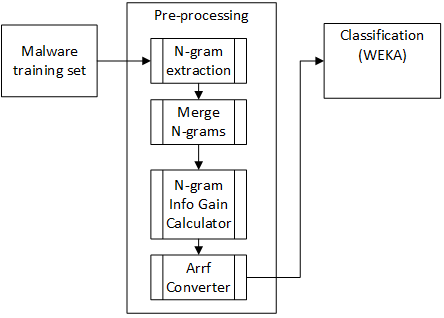
\includegraphics{system_architecture.png}}
	\caption{System architecture.}
	\label{fig:architecture}
\end{figure}

\subsubsection{Data Preprocessing}
The preprocessing part was a process that required a considerable effort because of the 
size of the training set, 10,868 files. The first step was to extract the hexadecimal
N-grams from the binary files using the kfNgram tool \cite{kfngram}, we used n=4.

It was then necessary to merge the resulting sorted N-gram files to effectively calculate the
\emph{information gain (IG)} of each N-gram. Because these files were extremely long,
we could not use the merge functionality built in the kfNgram tool, and we have to halt
the application after running for three days. To optimize this process we merged the files
maintaining a min-heap (or \emph{PriorityQueue} in Java) in memory with the first distinct N-gram 
from each file, as shown in Fig \ref{fig:merge_int}. We were also able to keep 10,878 Java
scanners in memory to speed up I/O. Then, to merging process would consist in each iteration
to perform a \texttt{pop()} operation from the \texttt{PriorityQueue}, append the element to merged
file, and insert the next N-gram from the same file of the element that was popped to the
\texttt{PriorityQueue}. This process is represented in Fig \ref{fig:merge_pop_replace}.

\begin{figure}
	\centering
	\scalebox{0.70}{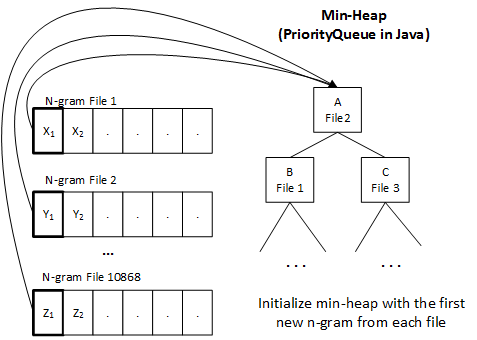
\includegraphics{merge_ngrams_init.png}}
	\caption{Initializing PriorityQueue to merge N-grams.}
	\label{fig:merge_int}
\end{figure}

\begin{figure*}[t]
	\centering
	\scalebox{0.70}{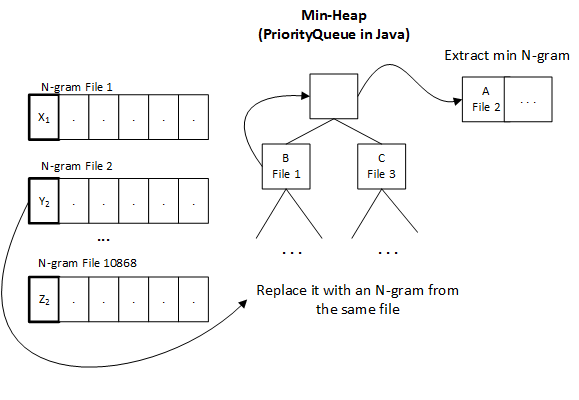
\includegraphics{merge_ngrams_pop_replace.png}}
	\caption{Process of merging N-grams. The minimum element is extracted and replaced with 
		another N-gram from the same file}
	\label{fig:merge_pop_replace}
\end{figure*}

Once merging was complete, we obtained a total of N-grams was 255,942,370, therefore we had to reduce 
them by calculating the  \emph{information gain (IG)} of each N-gram and selecting the top 500
(Fig. \ref{fig:info_gain_calc}), the same approach used in \cite{kolter:06}. The \emph{average mutual
	information} \cite{yang:97} was used to select the most relevant attributes:

\begin{equation}
	IG(j) = \sum_{v_j \in \{0,1\}} \sum_{C_i} P(v_j, C_i) \log \frac{P(v_j, C_i)}{P(v_j) P(C_i)}
\end{equation}

where \(C_i\) is the ith class,\(v_j\) is the value of the jth attribute, \(P(v_j, C_i)\) is the proportion that the jth
attribute has the value \(v_j\) in the class \(C_i\), \(P(v_j)\) is the proportion that the jth n-gram takes the value
\(v_j\) in the training data, and \(P(C_i)\) is the proportion of the training data belonging to the class \(C_i\) \cite{kolter:06}.

\begin{figure}
	\centering
	\scalebox{0.70}{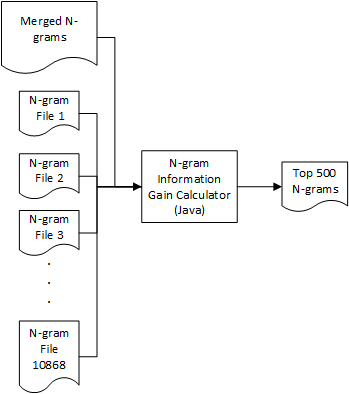
\includegraphics{N-gram_infogain.png}}
	\caption{Process of calculating the information gain of each N-gram.}
	\label{fig:info_gain_calc}
\end{figure}

The final step, as shown in Fig \ref{fig:ngram_arff}, in the data preprocessing was to transform the training set in .arff format where each example was represented by the presence (or absence) of the top 500 N-grams. This .arff file is one of the formats supported by Weka \cite{weka}, which facilitated to experiment with different machine learning algorithms.

Our system design for extracting the external API strings followed a near identical design, with the only difference being in the method use to parse the files (.asm) for the method calls. We used a simple shell-script that was designed to parse the files for any API methods using regular expressions. From there the we followed the same feature-set building pattern as for the n-grams.


\begin{figure}
	\centering
	\scalebox{0.65}{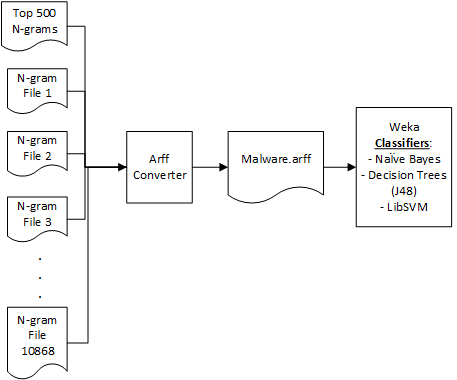
\includegraphics{n-gram_arff.png}}
	\caption{Transforming training set into .arff format.}
	\label{fig:info_gain_calc}
\end{figure}

\subsubsection{Classification algorithms}
\label{subsubsec:classif_alg}
The Naïve Bayes classifier uses Bayes' Theorem to label examples based on the assumption of conditional independence between features. Given a data set consisting of word counts, the training of this algorithm is very simple, and only requires the computation of the prior probability of each class, \(P(C_i)\), and the conditional probability of each word given a class, \(P(v_j|C_i)\). For a given instance \textbf{v}, we aim to classify it into some class, \(C_i\), thus computing \(P(C_i|v)\). Using Bayes' Theorem, this can be decomposed into:
\begin{equation}
	P(C_i|\mathbf{v}) = \frac{P(C_i) \ P(\mathbf{v}|C_i)}{P(\mathbf{v})} 
\end{equation}	
We can ignore the \(P(\mathbf{v})\) term, and estimate the remaining feature probabilities as:
\begin{equation}
	P(C_i) = \frac{\textrm{\# of occurences of class \textit{i}}}{\textrm{\# of total attributes}} 
\end{equation}
\begin{equation}
	P(v_j|C_i) = \frac{\textrm{\# of occurences of attribute } v_j \textrm{ with class }C_i}{\textrm{\# of occurences of class \textit{i}} }
\end{equation}
From here, we can define the classification of training example \textbf{v} as:
\begin{equation}
	\hat{y} = argmax \ P(C_k) \displaystyle\prod_{i=1}^n p(v_i \vert C_k)
\end{equation}


Decision trees are a method of classification that use tree-like graphs to model the classification of an example as a path of probabilities from the root node attribute, to one of the leaf (class) attributes. The beauty of decision trees lies in their simplicity and easy interpretation. Likewise, decision trees can be thought of as a "white-box" classification model, because once the tree has been built, the researchers can visualize and analyze each sub-path of an example's classification path.The basic implementation of a decision tree works as follows: for each node of tree, we select the attribute that best splits the our training examples into their respective classes using the entropy gain for choosing that attribute. For our system, we used the J48 decision tree algorithm in Weka, which is an implementation of the ID3 decision tree algorithm \cite{quinlan:86}. We define the entropy for a data set S, and its set of attributes V, as:
\begin{equation}
	H(S) = - \sum_{v \in V} P(v) \log_{2} P(x)
\end{equation}
Once we obtain the corresponding decision tree, we prune the tree to help minimize over-fitting that may have occurred as a result of tree's greedy construction.


Support Vector Machines (SVMs) produced the best classification results of our tested algorithms. The goal of an SVM is to find an optimal hyperplane that separates the training examples by their respective classes, while maximizing the margin between theses classes. The hyperplane is represented by a vector w and a scalar value b. Thus, the solution of the SVM can be represented by the minimzation of:
\begin{equation}
	P(\textbf{w},b,\boldsymbol{\xi}) = \frac{1}{2} \ \textbf{w} \cdot \textbf{w} + C \sum_{i=1}^{n}\xi_i
\end{equation}
such that:   
\begin{equation}
	\forall_{i=1}^{n} \ ,\ \xi_i \geq 0 \ : \ y_i(\textbf{w} \cdot \textbf{x}_i + b) \geq 1 - \xi_i
\end{equation}
where \(\mathit{\xi_i}\) is the upper bound on the number of training errors and \(C\) is the parameter that controls the trade-off between the margin of the hyperplane and the training error. We use the LibSVM \cite{chang:11} implementation of this algorithm. 

 We used pieces from two papers to design our system and framework. We expand the method of determining whether a given file is benign or malignant, i.e. whether or not it can be classified as malware \cite{kolter:06}. We also draw our n-gram extraction process directly from their paper. We used this feature extraction process to build our feature set which we then pushed through our algorithms. From <i>Learning and classification of malware behavior</i>, by K. Rieck et al, we derive our method of classifying malware into one of nine malware families. 


\section{Experimental Evaluation}
\label{sec:evaluation}
\subsection{Methodology}
Our experimental method blends the approaches of experiments in existing literature \cite{kolter:06,rieck:08}.We analyzed the system by running three machine learning classifiers on both of the feature sets we extracted- assembly and binary. The classification algorithms that we ran were the Naive Base Classifier, the Decision Tree ID3 algorithm, and the linear Support Vector Machine Classifier. The data we will present is our test error rate, Area Under the Curve (AUC), the precision and recall rates. All of these metrics were derived using 10-Fold cross-validation. We will delineate in the next section how these measurements relate to our ability to classify a malware file into one of the nine origin families. It is useful to determine the origin family of malicious file because each malware family describes their behavior and the damage they cause. This allows one to begin to diagnose and repair a machine. This information can also help one to prevent malware from executing undetected.  It also provides a road map for locating corrupted files and other deleterious deletions or insertions. 

We tested our method using 10,838 disassembled malware executables in both their binary and assembly formats, which we acquired from the Microsoft malware data set \cite{microsoft}. The information in this data set is compelling because it contains real-world viruses acquired and dissassembled by Microsoft. In addition, the data set is large enough to account for a wide variety of polymorphic changes to any of given malware family.  


\subsection{Results}
The results of our evaluation will show how the feature extraction methods outlined in the Kolter paper and the family classification methods in the Rieck paper are scaled, and how we replicated and improved upon their results. We had the most success with the accuracy of the SVMs for both the API strings and the n-gram feature sets as seen in Fig \ref{fig:results_table}. The error-rate analysis, AUC, precision and recall had the best results for both of these feature sets. These findings were in line with the cited literature and even showed improved results in regards to the Rieck paper.

Two of the stronger classifiers, SVM and Decision Trees, not only had improved accuracy for the n-gram approach but also a much smaller standard deviation which shows there is less variance in those results as compared to the API strings.

\begin{figure}
	\centering
	\scalebox{0.70}{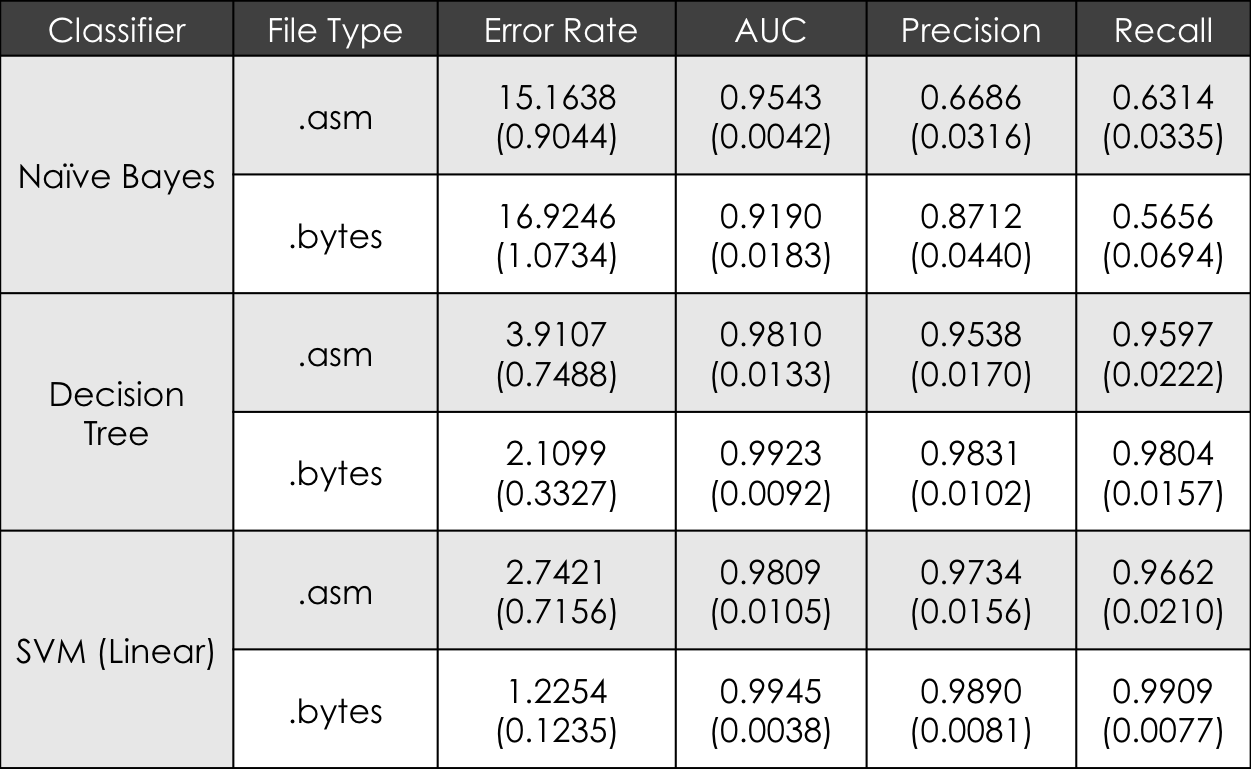
\includegraphics{results_table.png}}
	\caption{Experiment results (mean and standard deviation)}
	\label{fig:results_table}
\end{figure}

In Fig \ref{fig:class_acc_ngrams} and Fig Fig \ref{fig:class_acc_api}, the per-class accuracy of both methods was strongest for the linear SVM classifiers as well with the n-gram approach having all around better class accuracy results in general compared to the API strings method. We can attribute these findings to the fact that the API strings are not as unique a feature identifier as the n-grams.

\begin{figure}
	\centering
	\scalebox{0.70}{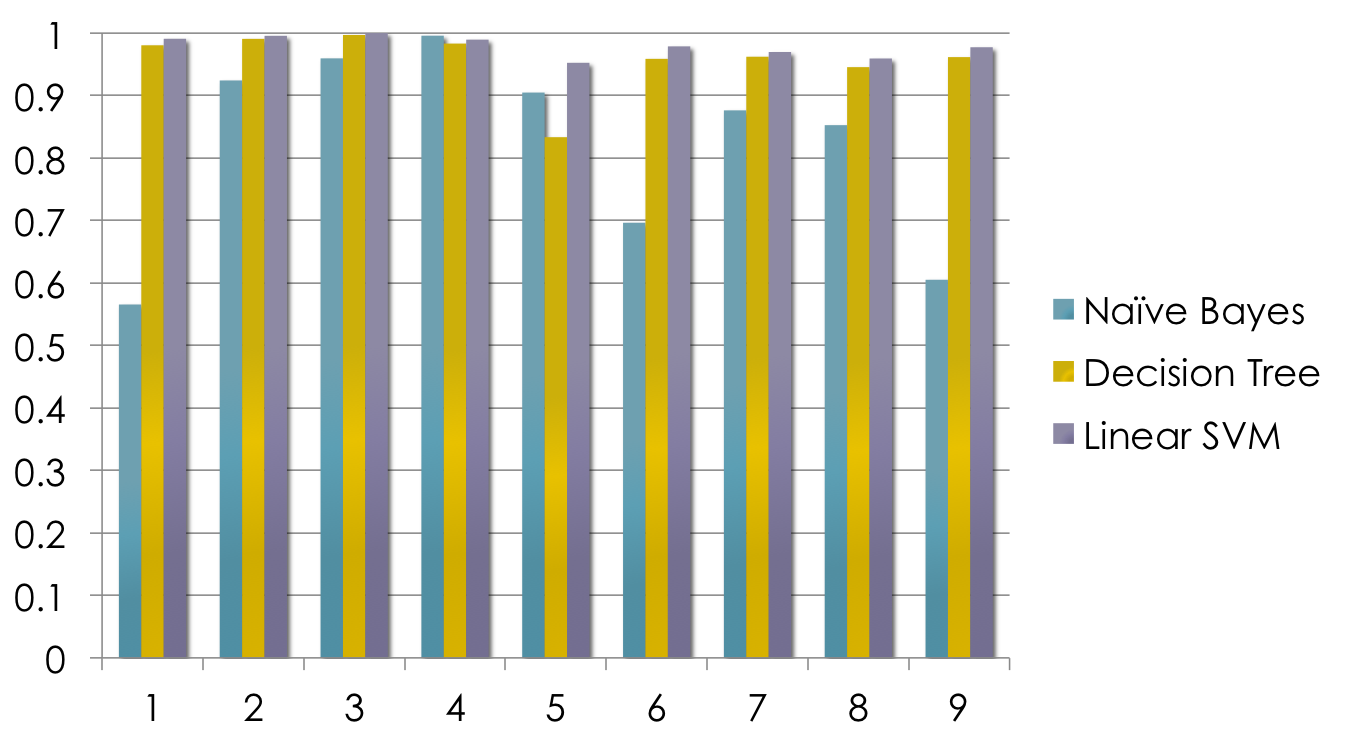
\includegraphics{class_accuracy_n-grams.png}}
	\caption{Family Accuracy using n-gram feature set}
	\label{fig:class_acc_ngrams}
\end{figure}

\begin{figure}
	\centering
	\scalebox{0.70}{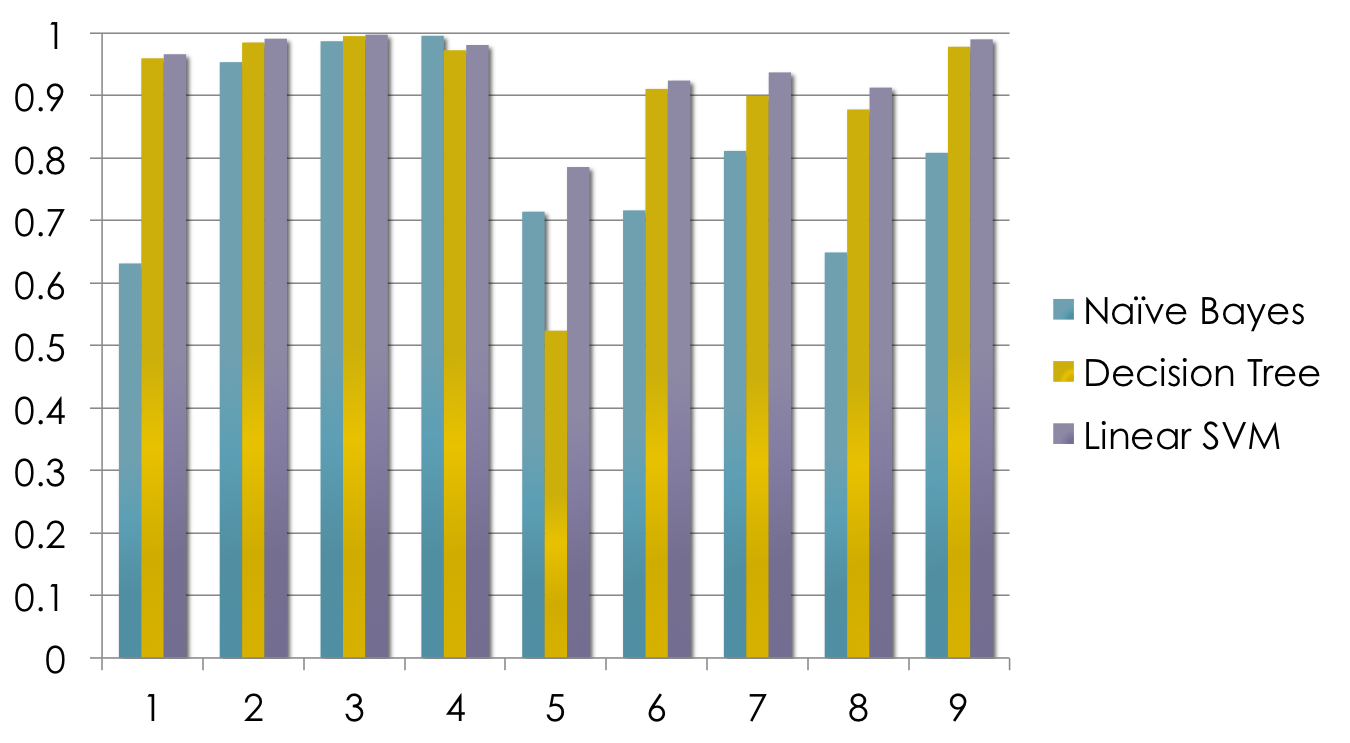
\includegraphics{class_accuracy_api-strings.png}}
	\caption{Family Accuracy using API strings feature set}
	\label{fig:class_acc_api}
\end{figure}

<<<<<<< HEAD
\subsection{Discussion}
\label{subsec:discussion}

Our results showed the importance of selecting the N-grams that would provide more information about the
underlying family by calculating the IG, instead of choosing the most frequent N-grams. With this method
we intuitively consider that irrelevant N-grams are avoided, which are those that are product of mutation
engines and other techniques used by hackers, and also we assume that by calculating the information gain
we somewhat extracted the most common instructions per malware family. This, we think, is the reason why 
we obtained a high accuracy with Decision Trees and Support Vector Machines, about 99\% in both. The
results are also inspiring in the sense that, at difference with other papers, our data set is considerable
large, and using several evaluation methods as cross-fold validation we presume we are not incurring in
overfitting.

This method is far from perfection, as there is still a considerable change of selecting irrelevant N-grams, 
which could have been mitigated by using sequential pattern extraction or Markov Models. The reasoning is
that the mutation engines, we believe, would not be capable of generating sequences of instructions that
would mislead the classification if we apply Markov Models or sequence pattern extraction correctly. 
=======
While the Rieck data set is comparable in size to the Microsoft data set, we achieved better accuracy and a better AUC measure. On average Rieck et al were only able to accurately classify 88\% of their sample file \cite{rieck:08}, where we were able to correctly assign 98\% to the proper malware family. Furthermore, where Rieck et al focus their work on a dynamic behavioral analysis of the API class, we focused our method on a more static paradigm, looking solely at the code contained within each malignant file. This dynamic behavioral modeling approach is not applicable to the average consumer and is therefore not as marketable. Whereas our detection system is transferable in the sense that it has real world applications. One only needs to run the file through a disassembler,such as IDA \cite{Eagel:08}, then parse the output for the n-grams or the API streams.  This can then be run through the SVM classifier, all of which can be done in real time and does not require the virtual sandbox environment that is required for the Rieck dynamic-behavior experiment.
>>>>>>> added section 3

%------------------------------------------------------------------------
\section{Related Work}
\label{sec:relatedwork}
%
Malware detection and classification is a problem being addressed through several angles. In \cite{oakland:2005}, 
the goal is to detect if a program exhibits a specified malicious behavior by determining if a set of templates of
sequence of instructions are present in the executable files. This approach requires to have knowledge on semantics
of each of the malware families. Although the results are promising, there are several reasons we could not follow
this approach, for example, as inferred by the title, it would be necessary to create a set of sequence of instructions
for each of the nine families we need to classify the malwares into. This is infeasible due to the length of the
course, but also it is outside of the scope of the course. As exhibited in the results, this strategy is resilient to
obfuscation and showed improvements when compared to McAfee VirusScan.

Several malware classification algorithms are based on n-grams extracted from the executable files. In \cite{securware:2011},
instead of byte sequences, the n-grams extracted are formed by machine codes. After obtaining the n-grams from the
malwares, a centroid for each family is created by selecting the most frequent n-grams. Then, the strategy to classify
a malware into one of the families, is to determine the centroid which the malware is more similar to by counting the
number of matching n-grams. When considering this approach, one of the possible limitations analyzed was that selecting
the most frequent n-gram could implicate choosing an n-gram irrelevant to the malware family.

We also explored sequential pattern extraction of n-grams. The proposed methodology in \cite{liangboonprakong:2013} 
outlines a procedure to use the n-grams patterns to classify the malware by family. The kfNgram tool \cite{kfngram} was
used to extract the n-grams from the disassembled files with n=1, n=2, n=3 and n=4, obtaining the best results with n=4. 
In \cite{kolter:06} the accuracy achieved was higher with n=4, therefore we skipped this evaluation and use only 
n-grams with n=4. The sequential pattern extraction technique in \cite{zhong:2012} was used to generate frequently 
occurred sequences of n-grams to represent the data \cite{liangboonprakong:2013}. Then the patterns significance 
was calculated using the term frequency-inverse document frequency (TF-IDF) where the term refers to the n-gram 
pattern and a document to the malware file. Since the number of patterns was too large, the sequential floating 
forward selection (SFFS) procedure was applied to reduce the number of features, in this case, n-gram sequential 
patterns. With all the features extracted, three classification algorithms were used, C4.5, multilayer perceptron 
and support vector machine. The training set was randomly split into two partitions using 80\% for training and 
20\% for testing achieving a 96.64\% of accuracy  \cite{liangboonprakong:2013}. Because of the duration of the 
course and the complexity of sequential pattern extraction, we were not able to experiment with this approach.

Following Occam's razor, suggesting that the simplest hypothesis is the best, we applied an approach similar to 
the one described in \cite{kolter:06}. The n-grams extracted from the executable files represented boolean features, 
present (i.e., 1) or absent (i.e., 0). Since the n-grams list was too large, it was necessary to select the most
relevant attributes (i.e., n-grams) by computing the \emph{information gain (IG)} described in \cite{yang:97} 
for each, also called \emph{average mutual information}. Through pilot studies, it was determined to use the 
top 500 n-grams, and then applied classifiers implemented in the Wakaito Environment for Knowledge Acquisition (WEKA) 
\cite{weka}: IBk, Naïve Bayes, SVM, and J48 (decision tree), and also \emph{boosted} the last three of these
learners \cite{kolter:06}. The results indicated 98\% the highest accuracy using boosted decision trees.



%-------------------------------------------------------------------------
\section{Future Work}
\label{sec:futurework}
Malware classification is a topic that is always evolving because viruses' 
authors are constantly developing techniques to avoid been detected, for 
example by obfuscating the code or by designing polymorphic behaviours. The 
proposed approach is agnostic of these techniques, therefore, we assume 
intuitively that a set of the extracted N-grams are product of this ingenious
methods. Mutation engines are capable of generating millions of variations of
the same virus, therefore, to overcome this problem, it would be necessary to
have knowledge of the malware behaviors to develop heuristics or detect specific
sequence of instructions to find in the malicious files.

For time reasons, we could not research on the possibilities of removing the
irrelevant computations in the malware files created to evade anti-viruses. This
would help, if using sequential N-gram patterns extraction, to detect patterns that
are truly correlated to the malware family. These patterns could, somewhat, describe
the common semantics present in each class of malwares.

\section{Conclusion}
\label{sec:conclusion}
%

%-------------------------------------------------------------------------
\subsection{Margins and page numbering}

All printed material, including text, illustrations, and charts, must be kept
within a print area 6-7/8 inches (17.5 cm) wide by 8-7/8 inches (22.54 cm)
high.



%-------------------------------------------------------------------------
\subsection{Type-style and fonts}

Wherever Times is specified, Times Roman may also be used. If neither is
available on your word processor, please use the font closest in
appearance to Times to which you have access.

MAIN TITLE. Center the title 1-3/8 inches (3.49 cm) from the top edge of
the first page. The title should be in Times 14-point, boldface type.
Capitalize the first letter of nouns, pronouns, verbs, adjectives, and
adverbs; do not capitalize articles, coordinate conjunctions, or
prepositions (unless the title begins with such a word). Leave two blank
lines after the title.

AUTHOR NAME(s) and AFFILIATION(s) are to be centered beneath the title
and printed in Times 12-point, non-boldface type. This information is to
be followed by two blank lines.

The ABSTRACT and MAIN TEXT are to be in a two-column format.

MAIN TEXT. Type main text in 10-point Times, single-spaced. Do NOT use
double-spacing. All paragraphs should be indented 1 pica (approx. 1/6
inch or 0.422 cm). Make sure your text is fully justified---that is,
flush left and flush right. Please do not place any additional blank
lines between paragraphs.

Figure and table captions should be 9-point Roman type as in
Figures~\ref{fig:onecol} and~\ref{fig:short}.  Short captions should be centred.

\noindent Callouts should be 9-point Helvetica, non-boldface type.
Initially capitalize only the first word of section titles and first-,
second-, and third-order headings.

FIRST-ORDER HEADINGS. (For example, {\large \bf 1. Introduction})
should be Times 12-point boldface, initially capitalized, flush left,
with one blank line before, and one blank line after.

SECOND-ORDER HEADINGS. (For example, { \bf 1.1. Database elements})
should be Times 11-point boldface, initially capitalized, flush left,
with one blank line before, and one after. If you require a third-order
heading (we discourage it), use 10-point Times, boldface, initially
capitalized, flush left, preceded by one blank line, followed by a period
and your text on the same line.

%-------------------------------------------------------------------------
\subsection{Footnotes}

Please use footnotes\footnote {This is what a footnote looks like.  It
often distracts the reader from the main flow of the argument.} sparingly.
Indeed, try to avoid footnotes altogether and include necessary peripheral
observations in
the text (within parentheses, if you prefer, as in this sentence).  If you
wish to use a footnote, place it at the bottom of the column on the page on
which it is referenced. Use Times 8-point type, single-spaced.


%-------------------------------------------------------------------------
\subsection{References}

List and number all bibliographical references in 9-point Times,
single-spaced, at the end of your paper. When referenced in the text,
enclose the citation number in square brackets, for
example~\cite{Authors14}.  Where appropriate, include the name(s) of
editors of referenced books.

\begin{table}
\begin{center}
\begin{tabular}{|l|c|}
\hline
Method & Frobnability \\
\hline\hline
Theirs & Frumpy \\
Yours & Frobbly \\
Ours & Makes one's heart Frob\\
\hline
\end{tabular}
\end{center}
\caption{Results.   Ours is better.}
\end{table}

%-------------------------------------------------------------------------
\subsection{Illustrations, graphs, and photographs}

All graphics should be centered.  Please ensure that any point you wish to
make is resolvable in a printed copy of the paper.  Resize fonts in figures
to match the font in the body text, and choose line widths which render
effectively in print.  Many readers (and reviewers), even of an electronic
copy, will choose to print your paper in order to read it.  You cannot
insist that they do otherwise, and therefore must not assume that they can
zoom in to see tiny details on a graphic.

When placing figures in \LaTeX, it's almost always best to use
\verb+\includegraphics+, and to specify the  figure width as a multiple of
the line width as in the example below
{\small\begin{verbatim}
   \usepackage[dvips]{graphicx} ...
   \includegraphics[width=0.8\linewidth]
                   {myfile.eps}
\end{verbatim}
}


%-------------------------------------------------------------------------
\subsection{Color}

Please refer to the author guidelines on the CVPR 2015 web page for a discussion
of the use of color in your document.

%------------------------------------------------------------------------
\section{Final copy}

You must include your signed IEEE copyright release form when you submit
your finished paper. We MUST have this form before your paper can be
published in the proceedings.

Please direct any questions to the production editor in charge of these
proceedings at the IEEE Computer Society Press: Phone (714) 821-8380, or
Fax (714) 761-1784.

{\small
\bibliographystyle{ieee}
\bibliography{egbib}
}

\end{document}
